% !TeX root = ams_thesis.tex
\chapter{System Development}

\section{Swarm Robot Hardware Platform}

Swarm robot platforms tend to fall into one of two groups, from a hardware perspective. 
The first group uses microcontrollers and very limited onboard computation, but is small and relatively cheap.
This group includes Alice, Jasmine, AmIR, and the other tabletop systems. 
Due to their limited computation, these systems do not generally support complex algorithms such as vision processing. 
The second group use more powerful computers, but at a significant cost in weight, power consumption, and financial outlay.

The robot described in this work is intended to occupy a theoretical ``sweet spot'' at the high end of the tabletop swarms or the low end of the room-scale swarms, depending on how large of a mobility platform is used. 
As a result, if it is configured for tabletop operation, the system can be used with a minimum of available space. 
If, on the other hand, it is configured for room-scale operations, the system can be tested in natural or naturalistic human environments. 

The robot swarm developed for this work consists of a hardware module for controlling two motors of a toy, such as a small RC car, for mobility. 
The reasons for choosing this hardware design are explained in more detail below, but the overall intent is to have an inexpensive platform available for swarm research, without having to rely on any particular group of swarm robotics researchers starting and maintaining a side business supporting and selling robots.
Duplication of software and other digital artifacts is trivial, so constructing a duplicate of the hardware becomes the primary difficulty. 
The use of toys for the mechanical components of the robots was intended to reduce the difficulty of constructing the hardware. 
If researchers are not to be expected to become entrepreneurs, they should also not be expected to become expert machine tool operators.
The hardware resulting from this work is designed so that it can be duplicated by a researcher using common tools, and possessed of no more than hobby-level familiarity with electronic hardware.

\begin{figure}
	\centering
	\includegraphics[width=0.8\textwidth]{../robot_makers_2/tiny_tank}
	\caption{A tank-drive toy with a 3.7V lithium polymer battery and a control board mounted to it.}
\end{figure}

In order to be both heterogeneous and inexpensive, the robots used for this work are constructed by developing a modular control hardware platform that can be attached to children's toys. 
Modified toys are an adequate substitute for custom mechanical assemblies, and permit easy experimentation with heterogeneous swarms. 
The controller module was designed to be used as a replacement for the control electronics of children's toys, similar to the Spider-Bots developed by Laird, Price, and Raptis, or Bergbreiter's COTSBots \cite{lairdspider, bergbreiter2003cotsbots}.
However, unlike the Spider-Bots and COTSBots, this work does not specify a particular toy chassis to use for mobility. 
Most children's toys use either one motor with a mechanical linkage to cause the toy to turn when the motor is reversed, or two motors.
Two-motor toys frequently use either differential steering or have one motor provide drive power and the other provide steering. 
All of these toys can be controlled by the hardware described in this work. 

The robots are intended to be heterogeneous, partly because of the advantages of heterogeneity in a swarm, and partly because toy supplies are unreliable.
While toys in the general case are expected to remain available, a particular line of toys might be discontinued or a modified version released. 
The software framework in development to support the robots is based on ROS, and so allows modular replacement of the control algorithms used to convert desired motion of the robot into drive signals for the motors. 

\begin{table}
	\begin{tabular}{l l l l l l l l }
		Name & Value & Cost (1) & Cost (100) & Count & Subtotal & Subtotal (100)\\
		\hline
		Battery & 3.7V & 3.41 & 1.5 & 1 & 3.41 & 1.5\\
		C1, C2 & 4.7uF & 0.5 & 0.2 & 2 & 1 & 0.4\\
		C3 & 0.1uF & 0.1 & 0.02 & 1 & 0.1 & 0.02\\
		C4 & 10uF & 0.19 & 0.06 & 1 & 0.19 & 0.06\\
		Charge IC & MCP73831 & 0.59 & 0.44 & 1 & 0.59 & 0.44\\
		Charge LED & Green & 0.54 & 0.3 & 1 & 0.54 & 0.3\\
		Diode & GF1A & 0.51 & 0.23 & 1 & 0.51 & 0.23\\
		Motor driver & DRV8830 & 2.27 & 1.64 & 2 & 4.54 & 3.28\\
		Header & 6-pin  & 0.52 & 0.37 & 1 & 0.52 & 0.37\\
		PCB &  & 3.3 & 0.79 & 1 & 3.3 & 0.79\\
		R1 & 470 ohm & 0.1 & 0.02 & 1 & 0.1 & 0.02\\
		R2 & 2k & 0.1 & 0.02 & 1 & 0.1 & 0.02\\
		R3, R4 & 0.22 ohm & 0.46 & 0.13 & 2 & 0.92 & 0.26\\
		R5, R8-12 & 10k & 0.1 & 0.01 & 6 & 0.6 & 0.06\\
		R6, R7 & 1k & 0.1 & 0.01 & 2 & 0.2 & 0.02\\
		Switch & 410-2016 & 0.91 & 0.72 & 1 & 0.91 & 0.72\\
		Thermal Fuse & 0ZB0050FF2G1 & 0.13 & 0.1 & 1 & 0.13 & 0.1\\
		V Regulator & MIC5265 & 1.4 & 1.06 & 1 & 1.4 & 1.06\\
		Wifi & ESP-8266-03 & 4.32 & 2.25 & 1 & 4.32 & 2.25\\
		\hline
		Total Cost &  &  &  &  & 23.38 & 11.9\\
	\end{tabular}
\end{table}

The mobility platforms used for the existing TinyRobo swarm cost 12-20 dollars in single quantities, putting the total cost for a single robot at \$35-45.
Where bulk ordering is available, the cost of 100 mobility platforms is \$8 per unit, reducing the per-unit cost of a 100-member TinyRobo swarm to \$20. 
This is roughly in line with the parts cost of the Kilobot, which is \$15 \citep{rubenstein2014kilobot}.

However, this should not be taken to mean that the TinyRobo platform is a competitor with the Kilobots. 
Kilobots were designed to have scalable interactions, which is to say that programming, charging, and even turning on the Kilobots does not take more time as the number of robots increases. 
To have programming take constant time, the Kilobots are programmed in parallel using an infrared broadcast device that illuminates the entire swarm at once. 
To charge together, the Kilobots have one charging contact on their legs, and the other on a leaf spring on their tops. 
By sandwiching the robots between two conductive plates, the entire swarm can be charged at once.
Finally, to all be turned on quickly, the Kilobots never turn off.  
Instead, they enter a low power sleep mode, and wake occasionally to check for an infrared signal to become fully active. 
This last attribute makes it very difficult to have a robot that has both wifi and a very low power sleep mode. 
The wifi module used in the TinyRobo platform consumes 15mA in its highest-power sleep mode, and 20$\mu$A in its lowest power mode. 
Unfortunately, only the highest power sleep mode can remain connected to an access point and receive a wake-up command, and so it will deplete the 750mAH battery used in the TinyRobos in just over two days. 
In contrast, a Kilobot can sleep for 3 months. 

The processor of the controller is an ESP-8266 wifi module.
The ESP-8266 costs approximately \$3-5, and contains both a wireless interface and a micro controller that can be programmed from a variety of programming environments and languages, including Lua and the Arduino variant of C/C++. 
The ESP-8266 module is based on the ESP-8266 IC, made by Expressif Systems. The IC itself has an 80Mhz Tensilica Xtensa L106 processor with 64kB of instruction memory and 96kB of data RAM. The modules come equipped with 512kB to 16MB of flash memory for program storage, and some combination of the 16 GPIO lines of the IC available for use. 
The ESP-8266 is available in several form factors, each designated by a different suffix. 
The version selected is the ESP-8266-03, which offers more GPIO pins than most other versions, and includes an internal antenna.

In addition to 802.11 b/g/n WiFi, the ESP-8266 supports a variety of serial protocols, including a UART, I$^2$C, SPI. 
The I$^2$C interface is used on the board to connect to two DRV8830 motor driver ICs by Texas Instruments. 
The DRV8830 provides 1A of drive current.
Experimental tests with 8 different toys indicate that small toys draw well under 1A while moving freely, and peak around 2A when the motors are stalled. 
The tested toys include 3 insect-styled walkers, 3 wheeled vehicles (2 differential drive, 1 Ackerman steering), 1 toy helicopter, and 1 toy quadcopter.
The DRV8830 provides overcurrent limiting, so a stall condition or short circuit of the motor leads will disable the motor drive, but not damage the DRV8830. 

The control module also provides connections for a 3.7V lithium-ion battery pack, as well as charge control circuitry for the battery. 
The charge controller allows the robot to be charged from the same USB connection that is used to change the programming of the ESP-8266. 
Reset and entry into programming mode is controlled by a separate USB-to-serial adapter board, the Sparkfun BOB-11736.
Moving this functionality to the adapter board reduces the size and cost of the control module. 

\subsection{Toy Compatibility} \label{section:Toy_Compatibility}

Children's toys normally use inexpensive brushed DC motors in their construction. 
These motors have not been the subject of extensive study, as they are commodity parts. 
However, it is useful to quantify their behavior to some extent, to determine which kinds of toys can be used with the controller. 

Two common types of motors found in children's toys are the RE and FA series of motors produced by Mabuchi Motor, or imitations of these motors produced by other companies. 
These motors use simple metal brushes and are constructed to be inexpensive, rather than precise. 
The intended voltage range of the motors varies with different winding types, but according to datasheets available from Mabuchi Motor, the voltage ranges and current draws for motors in this range are as shown in table \ref{tab:properBrandedMotors}.

\begin{table}
	\begin{tabular}{l l l l l}
		Model & Voltage & No Load Current & Max Efficiency & Stall Current\\
		\hline
		RE-140RA-2270 & 1.5-3 & 0.21 & 0.66 & 2.1 \\
		RE-140RA-18100 & 1.5-3 & 0.13 & 0.37 & 1.07 \\
		RE-140RA-12240 & 3-6 & 0.05 & 0.14 & 0.39 \\
		FA-130RA-2270 & 1.5-3 & 0.2 & 0.66 & 2.2\\
		FA-130RA-18100 & 1.5-3 & 0.15 & 0.56 & 2.1\\
		FA-130RA-14150 & 1.5-4.5 & 0.11 & 0.31 & 0.9\\
	\end{tabular}
	\caption{Current draw for Mabuchi-branded motors.}
	\label{tab:properBrandedMotors}
\end{table}

These motors have a volume of around 2cm$^3$.
For smaller toys, coreless motors are more common. 
The values in table \ref{tab:coreless} were measured from six of the toys used in constructing the swarm.
The measurements from the toy helicopter and toy quadcopter are included for comparison.
While the board can supply sufficient current to control all of these toys, it has not been tested in flying platforms.

\begin{table}
	\begin{tabular}{l l l}
		Motor number & No Load Current & Stall Current (measured)\\
		\hline 
		Hexbug brand mini spider & 0.03A & 0.13A (see caption) \\
		Hexbug brand 6-legged insect & 0.06A & 0.25A \\
		Miniature toy RC car & 0.21A & 0.8A \\
		Miniature toy RC insect & 0.19A & 1.13A \\
		Miniature toy RC vehicle & 0.37A & 0.8A \\
		Miniature toy RC vehicle & 0.06A & 0.74A \\
		Toy helicopter & 0.07A & 1.12A \\
		Toy quadcopter & 0.74A & 1.99A \\
	\end{tabular}
	\caption{No load and stall current for coreless DC micromotors. Measurements were performed at 3V supply voltage. The Hexbug mini spider includes a slip clutch, so attempting to stall the motors by holding the toy still does not prevent the motor from turning}
	\label{tab:coreless}
\end{table}


\subsection{Potential for Expansion} \label{section:Potential_for_Expansion}

The current design for the robots does not include sensors as a cost-saving decision. 
However, the communication between the ESP-8266 and the motor drivers uses the industry standard I2C bus serial interface. 
Due to the non-proprietary nature of this interface standard, it has been widely adopted, and many sensors are available to connect to an I2C bus. 
For example, Vishay Semiconductor makes the VCNL3020, which is an infrared proximity sensor with a 20mm range. 
If greater range is required, The ST Microelectronics VL53L0X Time-of-flight (ToF) laser ranger and gesture sensor provides a 2M range and 1D gesture sensing in a 4.4mm x 2.4mm package. 
As of this writing, the VCNL3020 is \$3.44 and the VL53L0X costs \$6.28 in single quantities.
These prices are reduced significantly when buying components in bulk, but because they increase the cost, size, and power draw of the hardware, they have not yet been integrated with this platform. 
Numerous multichannel ADC ICs with I2C interfaces are also available, which permits the addition of analog sensors to the platform. 

As a thought experiment, the cost of adding a 6-direction IR transmission and reception board to the TinyRobo platform was explored. 
This is not a finished design, but as much of the cost in a device of this type is in the semiconductors and PCB, it gives an estimate of the cost. 
The IR receiver selected would have been the TSOP5700TR, as used in the E-Puck Range and Bearing sensor board, but it is listed as obsolete by the manufacturer (Vishay Semiconductors). 
The modern replacement appears to be the TSMP6000.
The IR LED was also selected to match the E-Puck Range and Bearing board.

\begin{table}
	\begin{tabular}{l l l l l l}
		Part number & Cost (1) & Cost(100) & Count & Subtotal(1) & Subtotal (100)\\
		\hline 
		ATMega168 & 1.40 & 1.12 & 1 & 1.40 & 1.12  \\
		TSMP6000 & 1.81 & 1.03 & 6 & 10.86 & 6.18  \\
		SFH4255  & 1.06 & 0.59 & 6 & 6.36 & 3.54 \\
		SN74ACT08DR & 0.51 & 0.32 & 2 & 1.02 & 0.64 \\
		PCB & 3.3 & 0.79 & 1 & 3.3 & 0.79\\
		\hline 
		Totals & & & & 22.94 & 12.27\\
	\end{tabular}
	\caption{Semiconductors for a simple IR communication ring, and their prices. The PCB is the same size and type as the TinyRobo controller, and so has the same cost.}
	\label{tab:ir_ranger_board}
\end{table}

Colias appears to implement transmission power control for the infrared LEDs, and perform ranging by transmitting multiple times at varying power levels. 
If an object is detected by a low-power transmission, it is nearby, but if it is only detected by higher power transmissions, it is further away. 
Modulating the transmit power can also be used to limit range for inter-robot communication.
This modulation can be achieved using an AND gate which is powered from a digital output line of the main microcontroller, and applying a PWM signal to that output line.
Adding a 6-direction range and bearing board to the TinyRobo system could be expected to cost in the neighborhood of \$12-22 USD, depending on the quantity of boards produced. 

%Cooperative interaction of walking human and distributed robot maintaining stability of swarm 

%Development of IR-based short-range communication techniques for swarm robot applications 

%The Wanda Robot and Its Development System for Swarm Algorithms

%Stability of swarm robot based on local forces of local swarms

%Swarm robot pattern formation using a morphogenetic multi-cellular based self-organizing algorithm 

%A particle-swarm-optimized fuzzy-neural network for voice-controlled robot systems 

%The I-SWARM project 
% %
%\subsection{Current Consumption of Children's Toys} \label{section:Current_Consumption_of_Children_s_Toys}
%Motor driver test required, a well as quantification of motor current draw for children's toys. 
%Quantification of required power may indicate that larger motor driver power is needed.
% %
%Toys are effectively black boxes to the end user.
%Motors in particular are a commodity item, manufactured in large quantities without particular demand for electrical efficiency. 
%In the toys \improvement{Photos of motors and toys} used in this work, the most common motors are coreless brushed DC motors, although some of the larger toys also used brushed DC motors with cores. 
%The presence or absence of a core in the motor is of little practical concern in toys or in swarm robotic applications, as they are driven identically. 
% %
%All of the motors were driven at 3.7VDC. 
%This voltage was chosen because it is the output voltage of a fully-charged COTS lithium-polymer battery, which the platform uses for power. 
%Current was recorded for each motor running without the robot being in contact with the ground, to assess the minimum current draw, and stalled, to determine the potential maximum draw. 
%Current was measured using a multimeter, which does not have storage or recording capability, and so no attempt was made to determine peak surge current. 
% %
%Hexbug brand mini spider (two coreless brushed DC motors) Free run: 0.03A    Stall: 0.13A
%Hexbug brand 6-legged insect (one coreless brushed DC motor) Free run: 0.06A    Stall: 0.25A
%Miniature toy RC car, unknown model (one coreless brushed DC motor) Free run: 0.21A   Stall: 0.8A
%Miniature toy RC insect, unknown model (two motors, unknown construction) Free run: 0.19A    Stall: 1.13A
%Miniature toy RC car, differential steering (two motors, unknown construction) Free run: 0.37A    Stall: 0.8A
%Miniature toy RC vehicle, differential steering (two motors, unknown construction) Free run: 0.06A    Stall: 0.74A
%Toy helicopter (two motors, unknown construction, probably brushless) Free run: 0.07A   Stall: 1.12A
%Toy quadcopter (four motors, unknown construction, probably brushless) Free run: 0.74A   Stall: 1.99A

\subsection {Firmware}

The current version of the robots' firmware is developed in the open-source Arduino development environment.
Arduino programs are written in a dialect of C++. 

Every robot runs the same firmware. 
The firmware listens for connections on port 4321 for TCP/IP packets containing one of two types of messages. 
Messages starting with a 0x51 byte (ASCII `Q') cause the firmware to respond with a message containing the ASCII string ``TinyRobo". 
This function allows automatic detection of robots on a network by querying all connected systems to determine if they respond in this way. 

Messages starting with a 0x4D byte (ASCII `M') followed by four bytes are motor speed commands.
The firmware interprets the first two bytes as the speed and direction for the first motor, and the second two bytes as speed and direction for the second motor.
The control bytes are converted to a single byte command for the DRV8830 motor driver and transmitted over the I2C bus to set the motor speed.

The DRV8830 driver is a voltage-controlled motor driver. 
It accepts a single-byte command for each motor. 
Bits 7-2 of the byte define the output voltage to be applied to a motor, and the driver attempts to maintain that output voltage.
The valid range of motor voltage commands for the DRV8830 driver is 0x06 to 0x3F, which corresponds to a range of 0.48V to 5.06V in 0.08V increments. 
Because the robot battery is nominally 3.7V, the motor command 0x30 is the highest output available. 
Bits 1 and 0 of the command byte control the polarity of the output voltage, and so the direction of the motor, as per table \ref{tab:DRV8830_truth}.

\begin{table}
	\begin{tabular}{l l l l l}
		Bit 1 & Bit 0 & Out 1 & Out 2 & Function\\
		\hline
		0 & 0 & Z & Z & Coast\\
		0 & 1 & L & H & Reverse\\
		1 & 0 & H & L & Forward\\
		1 & 1 & H & H & Brake\\				
	\end{tabular}
	
	\caption{Truth table for DRV8830 drive direction bits. Coast allows the motor to turn freely. Brake connects the motor leads, which results in braking using the motor's back-EMF. Z indicates the output is in a high-impedance state}
	\label{tab:DRV8830_truth}
\end{table}

\begin{center}
	\begin{bytefield}[bitheight=\widthof{~Sign~},
		boxformatting={\centering\small}]{8}
		\bitheader[endianness=big]{7,2,0} \\
		\colorbitbox{lightred}{5}{Speed} &
		\colorbitbox{lightgreen}{2}{Dir}	
	\end{bytefield}
	%Can't caption here because this is outside float
	%\caption{Layout of bits in motor command byte for DRV8830}
\end{center}

Once the motor speed is set, the firmware reads the fault bytes from the DRV8830, and sends the motor command and the fault bytes for each motor back to the client over WiFi. 
The client uses the fault bytes to detect overcurrent conditions in the motor drivers and reduce output power. 

The decision to have all of the robots have the same firmware and control the speed of the motors from ROS was made because different toys have different control schemes. 
Toy tanks use differential drive, toy cars have Ackerman steering, and so forth. 
By moving the control to the main computer, the firmware can be kept simple while still allowing researchers to adapt the system to the available toys by modifying the software. 
 
\subsection{Why Heterogeneity?} \label{section:Why_Heterogeneity_}

Heterogeneity is a is a good model of many real-world systems where members of a group have different capabilities. 
Family groups of pack animals have young and old members, sometimes ill members, and sometimes infant members that cannot participate fully in pack activities. 
In human groups, work is divided according to ability, so a contractor may hire an electrician, a framing carpenter, and a plumber to build a house, to much better effect than attempting to do it with a team consisting entirely of plumbers. 

Another use of heterogeneity in swarms is to prevent individual robots from becoming overly complex by sparing them from having to be capable of doing everything. 
The presence of multiple robots with a given ability in a swarm strikes a compromise between all robots having that ability (and being complex and expensive) and only one robot having that ability (and so providing a single point of failure). 
Perhaps the most impressive recent demonstration of a highly heterogeneous swarm is the Swamanoid project's video ``Swarmanoid: The Movie", in which three different kinds of medium-sized robots cooperate to retrieve a book from a shelf \citep{oʼgrady2011swarmanoid}.
The movie explicitly mentions that one sub-team of robots (two mobile robots and one gripper robot) is positioned as back-up, in case the first sub-team fails. 

Beyond the possible utility of robots with multiple abilities, the swarm design presented in this work is heterogenous as a matter of convenience of implementation. 
As toys go out of production and are replaced by others, it may not be possible to continue to operate the swarm on an entirely homogeneous mobility platform. 
Because of this possibility, the software infrastructure tries to keep platform-specific calculations in a single module, and allow the rest of the system to operate using standard ROS messages. 
At present, these calculations only consist of conversion of ROS twist messages, which contain rotational and angular velocities in 3 axes each, into motor speed commands for the robot, which consist of a speed and direction for up to two motors. 

Handling the motion of the robots in this way means that the heterogeneity of the mobility platforms has a minimal impact on the conversion of user gestures into programs. 
However, as a direction for future work, it will become increasingly important to consider mobility as an aspect of program generation. 
For example, if the system is extended to include UAVs, and the user directs the robots to the center of a lake as part of a task, only the UAVs can be reasonably expected to reach the location undamaged. 
The system could be extended with some capacity for reasoning about the task environment, to determine how the capabilities of the robots interact with that environment. 
Such an augmented system could then refuse to direct ground robots into water, and report if there are not a sufficient number of aerial robots to perform the task over the lake. 
It could also permute task assignments based on robot capabilities in order to meet other goals, such as minimizing the number of robots used or maximizing available robot battery life. 

\section{Swarm Robot Software Framework} \label{section:Swarm_Robot_Software_Framework}

The individual robots being developed for this research have minimal sensing capacity and relatively weak processors. 
The majority of the processing is performed on a host computer running the ROS software framework. 
Each robot's processor is mostly concerned with controlling the motors of the robot. 
The structure of the software framework is such that as available processing power on each individual robot increases, more of the processing can be handled locally, without changing the overall design of the system.

The central computer has a top-down camera over the ``arena'' the robots are active in. 
Each robot has an AprilTag on top of it, so that the central computer can localize them within the arena \citep{olson2011tags}. 
The central computer uses the location information to create ``virtual sensors'' for each robot. 
Since the central computer knows the location of each robot, the relevant information can be sent to each robot's control process as if it were coming from a sensor on the robot. 
For example, a range and bearing sensor that allows each robot to detect the distance and angle of the nearby robots is simple to implement in software. 
Range and bearing sensor functionality is available in hardware on E-pucks and Marxbots, but since each robot must be equipped with it, the cost scales linearly with the number of robots to equip.  
It is possible to calculate the odometry for individual robots by watching the change in position in their tags over time. 
The calculated odometry could then be published as a ROS topic, just like odometry collected from e.g. wheel encoders. 
The virtual sensors can also be configured to emulate error conditions such as noisy sensors, failed sensors, degraded localization, and so forth.
Virtual parameter tweaking allows fine-grained testing of the behavior of algorithms under imperfect conditions, and the response of human users to unreliability in the swarm. 

%Graphic of the software environment as a whole
\begin{figure}[h]
	\centering
	\digraph[scale=0.6]{Framework}{
	
	graph[nodesep=0.5];
	
	subgraph clusterRobot1 {
		motor[shape=box; label="Motor Driver"];
		robotCode[label=<Robot <br/> Firmware>];
		robotCode -> motor;
		label="Robot 1";
		shape=box;
	}
	
	subgraph clusterRobot2 {
		motor2[shape=box; label="Motor Driver"];
		robotCode2[label=<Robot <br/> Firmware>];
		robotCode2 -> motor2;
		label="Robot 2";
 		shape=box;
	}
	
	subgraph clusterRobot3 {
		motor3[shape=box; label="Motor Driver"];
		robotCode3[label=<Robot <br/> Firmware>];
		robotCode3 -> motor3;
		label="Robot 3";
		shape=box;

	}
	
	subgraph clusterRobotN {
		motorN[shape=box; label="Motor Driver"];
		robotCodeN[label=<Robot <br/> Firmware>];
		robotCodeN -> motorN;
		label="Robot N";
		shape=box;
	}
	
	subgraph clusterComp {
		concentrate=true;
		label="Control Computer";
		{rank=source;
			vrSense [label="Virtual Sensors"];
			vrNet [label="Virtual Network"];
			worldModel [label="World Model"];
			worldModel -> vrSense;
			worldModel -> vrNet;			
		}
		rp1 [label=<Robot <br/> Process 1>];
		rp2 [label=<Robot <br/> Process 2>];
		rp3 [label=<Robot <br/> Process 3>];
		rpN [label=<Robot <br/> Process N>];
		vrNet -> {rp1, rp2, rp3, rpN} [dir="both"];
		vrSense -> {rp1, rp2, rp3, rpN};	
	}
	
	camera[label=<Overhead<br/>Camera>;shape=box;]
	camera->worldModel;
	
	rp1 -> robotCode [label="WiFi", dir="both"];
	rp2 -> robotCode2 [label="WiFi", dir="both"];
	rp3 -> robotCode3 [label="WiFi", dir="both"];
	rpN -> robotCodeN [label="WiFi", dir="both"];
	}
	\caption{Overview of the planned framework. Rectangular nodes are hardware, oval nodes are software.}
\end{figure}

Since the robots are reporting to a central server, and the central server also receives the video from the overhead camera, it may appear that this is a highly centralized system. 
However, the central computer provides a framework for implementing a decentralized control scheme on the individual robots. 
Rather than controlling each robot, the central computer maintains a separate process for each robot in the swarm. 
Each of these robot processes only has access to the information that would be available to that robot, based on its physical location, and so acts as a local control program for the robot, but with the full processing resources of the host computer. 
As a result, the individual robots can be small, lightweight, and consume relatively little electrical power, but the system as a whole gives them significant computing power. 
When more powerful and lower power consumption processors become available, more of the processing can be moved from the virtualized robot processors and onto the actual robots, enabling a smooth transition from a simulated decentralized system to a real decentralized system. 

\subsection{Virtual Localization} \label{section:Virtual_Localization}

The AprilTag tracking of the robots provides localization of the robots within a common coordinate frame. 
It should be stressed that while the central computer can localize the robots, both relative to each other and by absolute position within the arena, this information may be withheld from the individual robots, or given to them if required. 
The code virtually operating on the robot may be neither aware of its own position in the world, nor the location of other robots, if the experiment calls for such a lack of information. 

Currently, the AprilTag-based localization is used to implement virtual laser scanners similar to the Sick or Hokyuo brand laser scanners used on larger robots. 
It is also used to limit the range of messages sent between the robots through a virtual network. 

\subsection{Virtual Laser Scanners} \label{section:Virtual_Laser_Scanners}

The AprilTag localizations and the image of the arena are used to provide virtual laser rangers for each robot. 
The virtual laser ranger consists of two ROS nodes, a service and clients for the service. 
The service is called ``laser\_oracle\_server''. 
It subscribes to the AprilTag detections and the images from the arena overhead camera. 
 
When a client requests a laser scan, the virtual laser service masks the modified arena image with a circle with a radius of the laser range, centered on the robot requesting the scan.
This masking removes all of the objects that are out of range of the laser, and so reduces the time spent calculating the laser scan points. 

Each sample of the laser scan is represented as a line segment, located based on the requested start, stop and inter-measurement angles for the virtual laser scanner. 
Each line segment is checked for intersection with the lines defining the contours of the blue objects in the image. 
As the virtual laser service receives images, it draws a blue dot over the location of every robot. 
This dot provides the outer edge of each robot in the virtual laser scan. 
The approach of using blue objects as obstacles was chosen because if the laser scanner service treats anything blue as an obstacle, then ``walls'' can be created in the arena by making lines of blue masking tape on the arena floor. 
If multiple intersections are found for a line segment, the intersection closest to the robot is used, as the laser would stop after reflecting off an object.
The service then formats the distances to the intersection points as a ROS sensor\_msgs/LaserScan and returns it as the service response to the requesting client. 

The virtual laser clients take the place of the laser driver ROS nodes that would be used to control a real linear laser scanner. 
The laser client is initialized with some parameters, such as the sweep angle and angular resolution of the virtual laser, and polls the laser service regularly. 
As it receives laser scans from the service, it publishes them to a ROS topic in the same manner as a ROS node for a hardware laser. 

The apriltags\_ros node publishes the detected locations of the tags in meters, but the computer vision detection of blue objects in the arena camera image operates in pixels. 
In order to convert from pixels to real-world distances, the apriltags\_ros node was forked and a modified version was created that provides the locations of the tags in pixel as well as real-world coordinates. 
The modified version is available at https://github.com/ab3nd/apriltags\_ros.

\begin{figure}
 	\centering
	\digraph[scale=0.6]{VirtualLaserSystem}{
	
	vls -> vsc [label=<std\string_msgs/Integer&nbsp;&nbsp;&nbsp;&nbsp;>];
	vsc -> vls [label=<sensor\string_msgs/LaserScan>];
	vsc -> sub1 [label=<sensor\string_msgs/LaserScan>];
	cam -> vls [label=<sensor\string_msgs/Image>];
	cam -> atag	[label=<sensor\string_msgs/Image>];
	atag -> vls [label=<apriltags\string_ros/TagDetections>];	
		 
	vls [label="Virtual Laser Service"];
	vsc [label="Virtual Laser Client"];
	atag [label="AprilTag Detector"];
	cam [label="Arena Camera"];
	sub1 [label="Subscriber"];
 	}
	\caption{Data flow in the virtual laser service}
\end{figure}

\subsection{Virtual Networking} \label{section:Virtual_Networking}

If the robots are required to communicate directly with each other, the communication passes through a virtual network.
From the point of view of the robots, messages sent into the virtual network are delivered to other robots as if the messages were sent directly from one robot to another. 
However, all the communication is taking place between processes running on the central computer.
By changing how the messages are delivered by the central system, the virtual network can provide full connectivity, range-limited mesh networking, directional beacons, or other forms of networking. 
The reliability of the network can also be varied, by dropping some messages or otherwise changing them based on information about the robots. 
For example, the likelihood that a message arrives at the robot to which it was transmitted may depend on the distance between the sender and receiver.
Signals that pass through a virtual wall may have a reduced virtual signal strength and range.

 \begin{figure}
 	\centering
	\digraph[scale=0.6]{VirtualNetwork}{
	
	{rank=same atag dist}
	{rank=same tx rx}

	vns -> dist [label="Robot IDs"];
	dist -> vns [label="Distance"];
 	cam -> atag	[label=<sensor\string_msgs/Image>];
	atag -> dist [label=<apriltags\string_ros/TagDetections>];	
	vns -> rx [label="Network Message"];
	tx -> vns [label="Network Message"];	 
	
		
	vns [label="Virtual Network Service"];
	dist [label="Distance Service"];
 	atag [label="AprilTag Detector"];
 	cam [label="Arena Camera"];
	tx [label="Transmitter"];
	rx [label="Receiver"];
 	}
	\caption{Data flow in the virtual network. The virtual network service can take the distance between the transmitting robot and the receiving robot into account when determining if the message is delivered.}
 \end{figure}

\section{Swarm Hardware Results} \label{section:The_Desert_of_the_Real}

Due to mechanical flaws in the toys used as motion platforms in TinyRobo, the robots would sometimes not move as commanded (see figure \ref{motor-speed-fig}). 
In a single-robot system, transient failures can sometimes be accommodated by repeated effort or replanning. 
However, in a multi-robot system the scale of the system works to offset the reliability of each individual robot. 
If robots have an individual mean time between failures (MTBF), the expected mean time to any failure is the MBTF divided by the number of robots. 
For example, if an individual robot can work for 100 hours between failures, it would be reasonable to expect it to work for at least a day. 
However, if the swarm consists of 1000 such robots, a failure of at least one robot can be expected within 6 minutes. 
Tracking the failure of existing platforms in the field placed the average MBTF of commercial mobile platforms at 24 hours, with indoor robots fairing much better than outdoor ones \citep{carlson2004follow}.


\begin{figure}[t]
	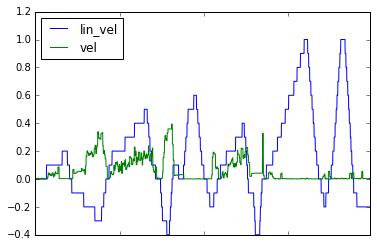
\includegraphics{motion_vs_cmd}
	\centering
	\caption{Commanded velocity (lin\_vel) as opposed to recorded motion (vel). Vel is always positive because it is measured in terms of euclidian distance moved by the center of the AprilTag between successive updates of the tag tracking. 
		Note that while the magnitude of the motion is proportional to the commanded motion, sometimes the robot did not move at all, and when it did move, the recorded velocity is quite noisy. Noise may be removed in software, mechanical failure cannot.} 
	\label{motor-speed-fig}
\end{figure}

This problem was highlighted by the use of inexpensive toys. 
It is desirable to have a swarm platform be able to run for extended periods, in order to acquire data for experiments. 
Toys, especially cheap ones, are designed for low cost and an MBTF more compatible with the attention span of children than that of researchers. 
The amount of effort devoted to locating and eliminating mechanical problems relative to the runtime of the system was not acceptable.

\subsection{Calibration} \label{section:Calibration}

Children's toys are prone to failure and inaccuracy.
In toys, particularly remote controlled toys, the user acts as a the feedback element of a control system, observing the behavior of the toy and changing their actions as a result. 
If an individual toy, for example, has a bias to turn to the left, the user will learn this and apply a correcting bias.
To extend this to a computerized system requires some form of calibration. 
These calibration steps, combined with appropriate control, such as PID loops, can account for systemic inaccuracies. 
However, the use of toys also introduces some failures which are not consistent or linear. 
For example, the tanks used in some instances of the TinyRobo platform use motors with high speed, but relatively low torque. 
As a result, dirt in the drivetrain near the motor can cause the motor to become difficult to start, but can be removed by the user, or by operation once the motor does start. 
Calibration when the dirt is present means the robot will start very abruptly when the dirt is removed, while calibration when the dirt is absent means the robot may not start if dirt gets into it later. 
It is worth noting, in light of this example, that GritsBots, Kilobots, and mROBerTO all use nearly-sealed drivetrains, either direct motor drive of the wheels or sealed vibration motors \citep{rubenstein2014kilobot, Kim2016mROBerTOAM, pickem2015gritsbot}. 

An early intent of the author was to have the system learn the control law for each robot through observation of the relationship between the commanded motion of the robot and the resulting motion. 
Due to the overarching concern with human control of a swarm, such online calibration was decided to be out of scope for this work. 
However, a computer-vision-guided calibration technique was used in the mROBerTO swarm robots to compensate for manufacturing differences between robots \citep{Kim2016mROBerTOAM}. 

This approach results in learning bad controls if the system observes the robot during a temporary failure. 
In a system with minimal failures, this problem can be minimized, but as discussed earlier, inexpensive children's toys are not such a system. 

GRITSBots have a calibration step, but the calibration is automated, and is only performed once for each robot, after which it is assumed that the calibration variables are constant.
Calibration can be automated in a homogenous platform with reasonably reliable hardware. 
Non-homogenous platforms require different calibration for different platforms, which reduces the benefit of automation. 
Further, requiring calibration works against transitioning to a new platform by adding an additional hurdle in the form of developing a new calibration method.

The lack of an automated calibration and control method drove the TinyRobo swarm to use more differential drive vehicles, as they struck a balance between the fully holonomic drive used in the SpiderBots, which is expensive but easy to control, and the Ackerman drive used in inexpensive RC cars, which is less expensive, but has more complex control math \citep{lairdspider}.
It also increases the difficulty of using a heterogenous system, and so operates against the advantages of heterogeneity as discussed in section \ref{section:Why_Heterogeneity_}

%\subsection{April Tag Latency} \label{section:April_Tag_Latency}
%
%April tags have very solid position and orientation tracking, but are computationally intensive to detect and localize in typical webcam images. 
%More tags leads to longer computation time, increasing the latency of the robot control loop. 
%Parallelizing the implementation of the AprilTag library could improve it significantly, but is out of scope for this work. 
%
%One version of the GRITSBots used AprilTags and a standard web cam, resulting in position updates at approximately 10Hz. 
%This update rate is consistent with that observed by the author using the ROS implementation of AprilTags. 
%Decreasing the size of the image in which the tags are detected speeds it up, at the cost of requiring larger tags in order to have them legible in the lower-resolution image. 
%The update rate places an upper bound on the ability of the system to respond to the motion of the robots. 
%To decrease the latency of this sensing, the GRITSBots team considered moving to color blob tags, which can be detected by the onboard vision processor of a Pixy CMUCam5 at up to 50Hz \citep{PickemGrits2014}. 


\subsection{Drive Testing} \label{section:Drive_Testing}

In order to characterize the behavior of the various toy hardware that the TinyRobo platform could be used on, seven TinyRobos were commanded by a program which instructed them to move forwards until the AprilTag tracking determined that they had moved a fixed distance, stop, and move again, in a loop. This program was run until the robot failed to move or ran into the walls of the robot arena.

Each robot was run 5 times, starting from the same location each time. The robot was power-cycled between runs. Each run was recorded using rosbag, and the data from the recordings were used to generate visualizations of the robot's commanded trajectory from the motion of the center of the robot's AprilTag.

The robots consisted of three toy tanks from the same manufacturer, a differential-drive Hexbug-brand robot, a differential-drive toy car with large wheels, a hexapod bug-like walker, and an Ackerman-drive toy car. 
The bug-like walker and the Ackerman-drive car both have different turning kinematics from the differential drive tanks, but this test only consists of forward drive.
It would have been preferable to have the test include turning, but control of the yaw rotation of a robot via feedback from the AprilTag system was found to be problematic. 
As the number of pixels that an AprilTag takes up on a camera image decreases, the accuracy of the subpixel estimation used to localize the corners of the tag decreases. 
Each estimation of the tag location from the ROS AprilTag detection node can then differ from previous estimations, and so even when the robot remains still, there is some noise in its detected position. 

The effect of the noise in subpixel position on the perceived rotation of the tags is larger than its effect on the perceived rotation of the tags, since rotation around the center of the tag does not change the position of its center at all. 
As a consequence, the tags could be detected to be in lateral motion by comparing the displacement of the center of the tag and checking that it was greater than the expected noise, but detection of rotational motion and velocity calculation was sometimes swamped by noise. 

The noise was also determined to be unevenly distributed over the robot arena. Because the arena is wide, a 140$^{\circ}$ wide-angle lens is used to ensure that the entire arena is visible. 
ROS provides tools for removing the distortion inherent in the use of a wide-angle lens, but at the cost of decreased effective resolution at the edges of the image. 
This decrease in resolution results in reduction of subpixel location accuracy, and so increased noise in localization of the tag at the edges of the arena closest to the edges of the camera image. 

Because the desired figure-8 motion could not be performed with the rotational localization noise present in the system, the robots were instead commanded to move forward 0.25m, stop, and repeat that sequence of actions until the program was stopped. 
The program was stopped if the robot was about to run into the wall of the arena, or had entered a state in which it could not move forward anymore. 
Acceleration during the movement phases was managed by increasing the commanded velocity of the robot until the AprilTag tracking detected that the robot had begun moving. 
Once the robot began moving, it was not commanded to change velocity until it had moved at least 0.25m.
In the following descriptions of the motions of the robots, the directions left and right are relative to the direction of travel of the robot. 

The Ackerman-steering toy car (page \pageref{img_traj}, image a) displayed very consistent mobility. In four out of its five runs, it crossed the arena without incident. 
In one run, it started and went a small distance, but then did not start again. 
However, the Ackerman-steering toy car has a gearbox that permits backdriving, so when commanded to stop, it coasts for a few centimeters. 
The toy tanks use a worm gear in their drivetrains, and so do not permit backdriving of the motors by the vehicle's inertia. 
Instead of coasting, they immediately stop when the motor is commanded to 0 velocity. 

The big wheel robot (page \pageref{img_traj}, image b) displayed an unfortunately small range of commanded velocities between those which caused it to begin moving, and those which caused it to flip over on its side.
In three of its five runs, the big wheel accelerated quickly and then flipped during the first motion period. 
In the remaining two runs, it did not move at all, possibly due to gears jamming. 

\begin{figure}
	\centering
	\begin{subfigure}[t]{0.3\textwidth}
		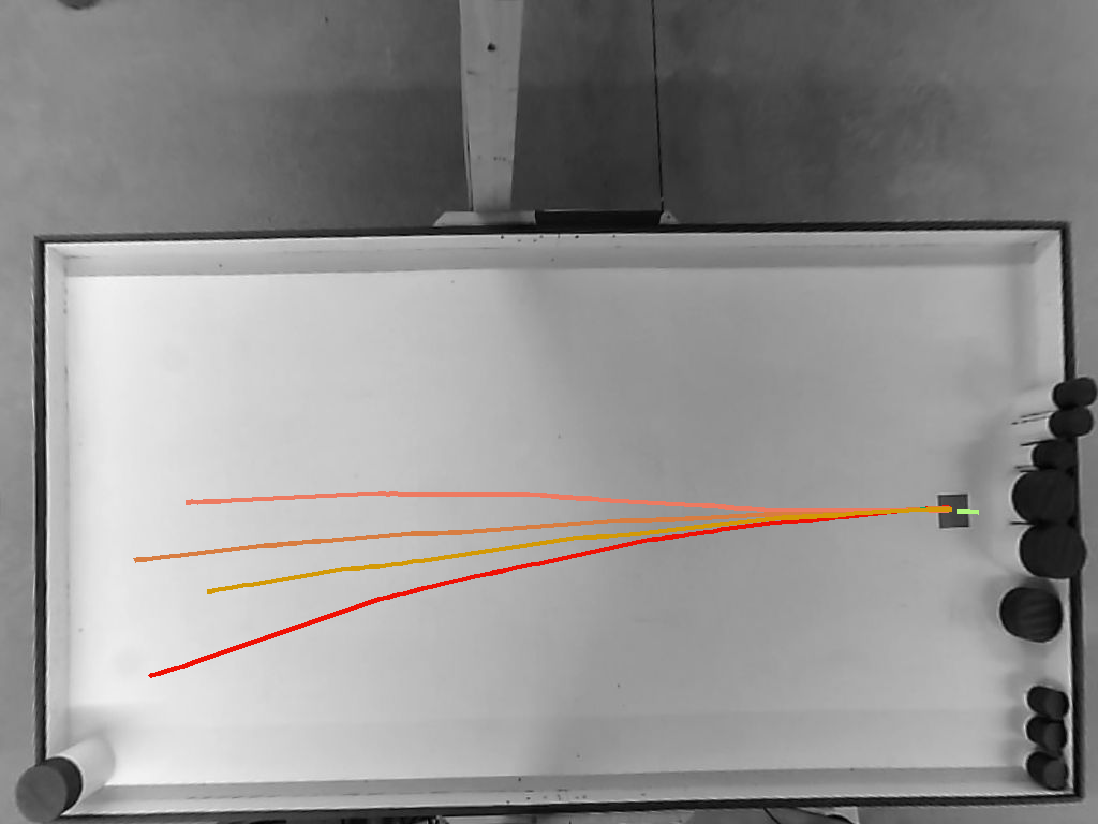
\includegraphics[width=\textwidth]{../hardwareX_paper/robot_17.png}
		\caption{Motion of toy car based robot}
	\end{subfigure}
	\begin{subfigure}[t]{0.3\textwidth}
		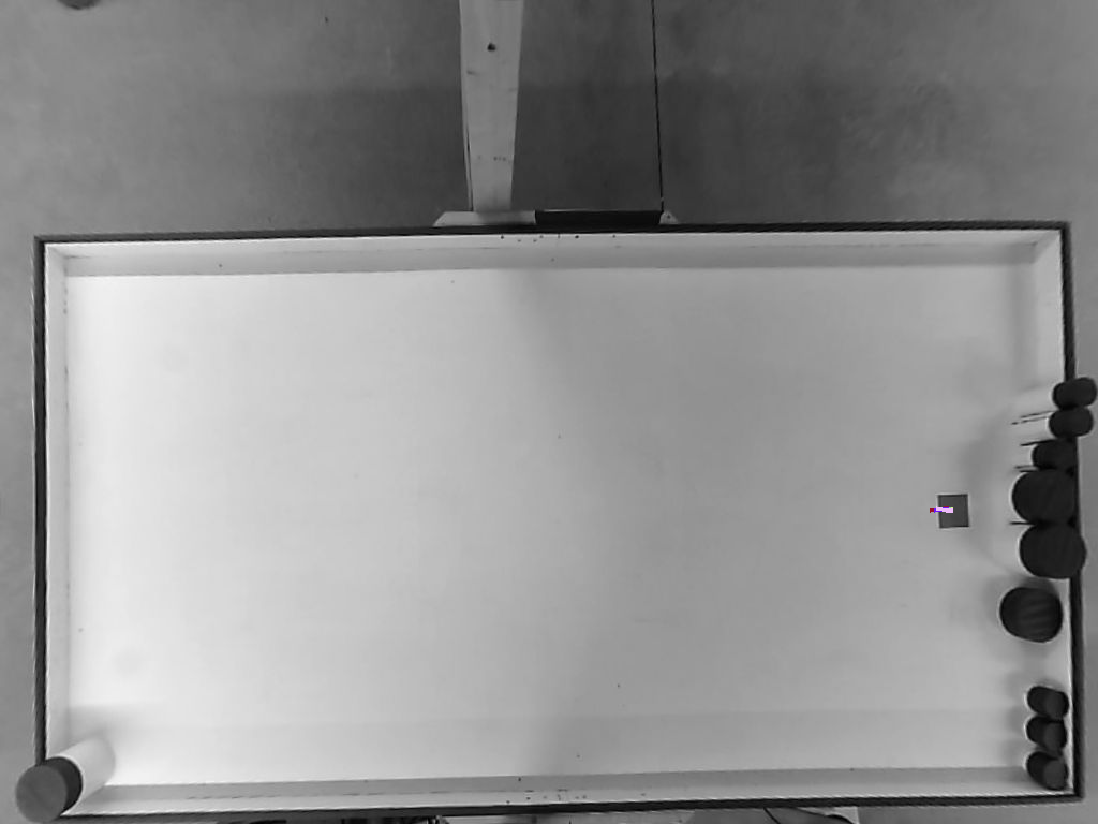
\includegraphics[width=\textwidth]{../hardwareX_paper/robot_1.png}
		\caption{Motion of big wheel robot}
	\end{subfigure}
	\begin{subfigure}[t]{0.3\textwidth}
		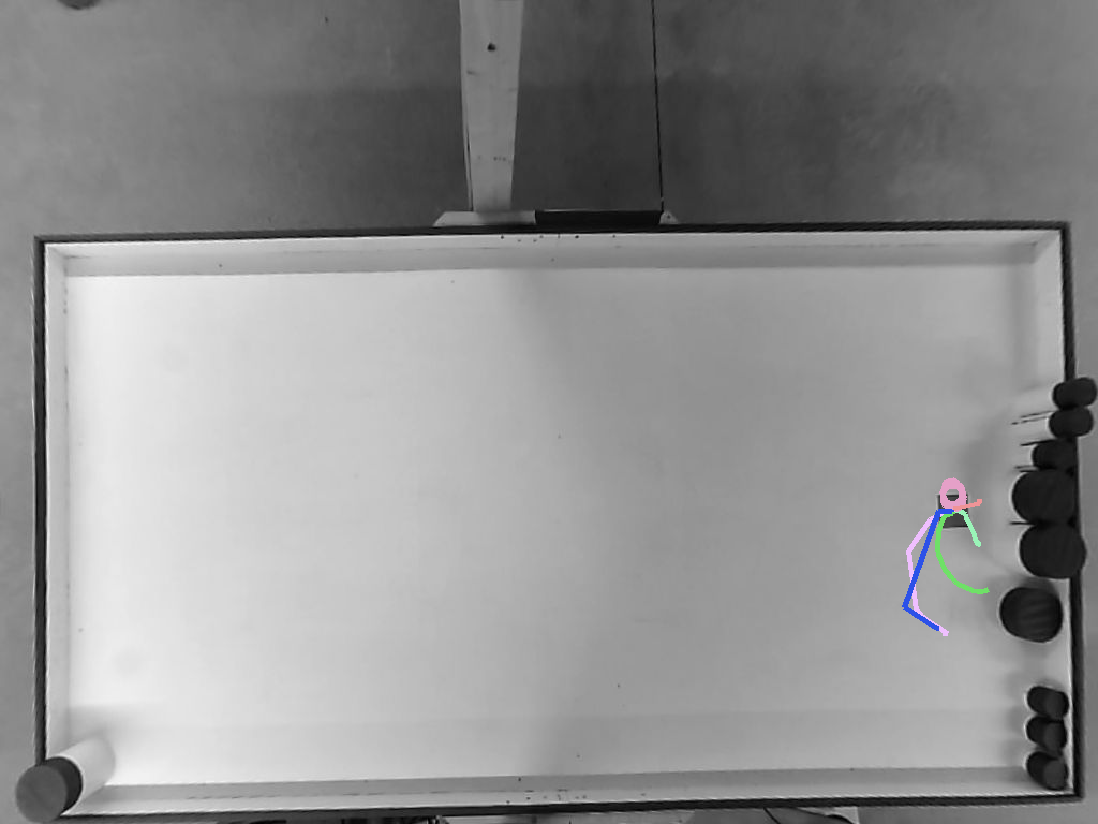
\includegraphics[width=\textwidth]{../hardwareX_paper/robot_6.png}
		\caption{Motion of 6-wheel bug}
	\end{subfigure}
	
	\begin{subfigure}[t]{0.3\textwidth}
		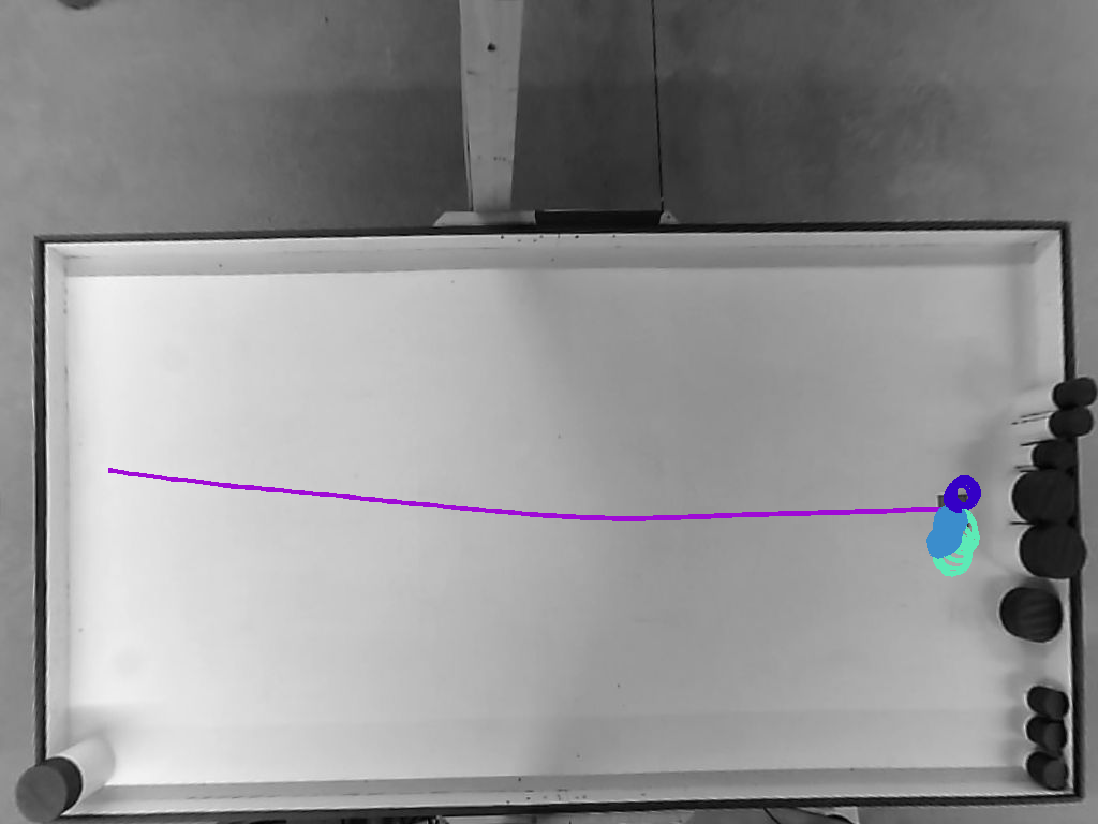
\includegraphics[width=\textwidth]{../hardwareX_paper/robot_0.png}
		\caption{Motion of green tank}
	\end{subfigure}
	\begin{subfigure}[t]{0.3\textwidth}
		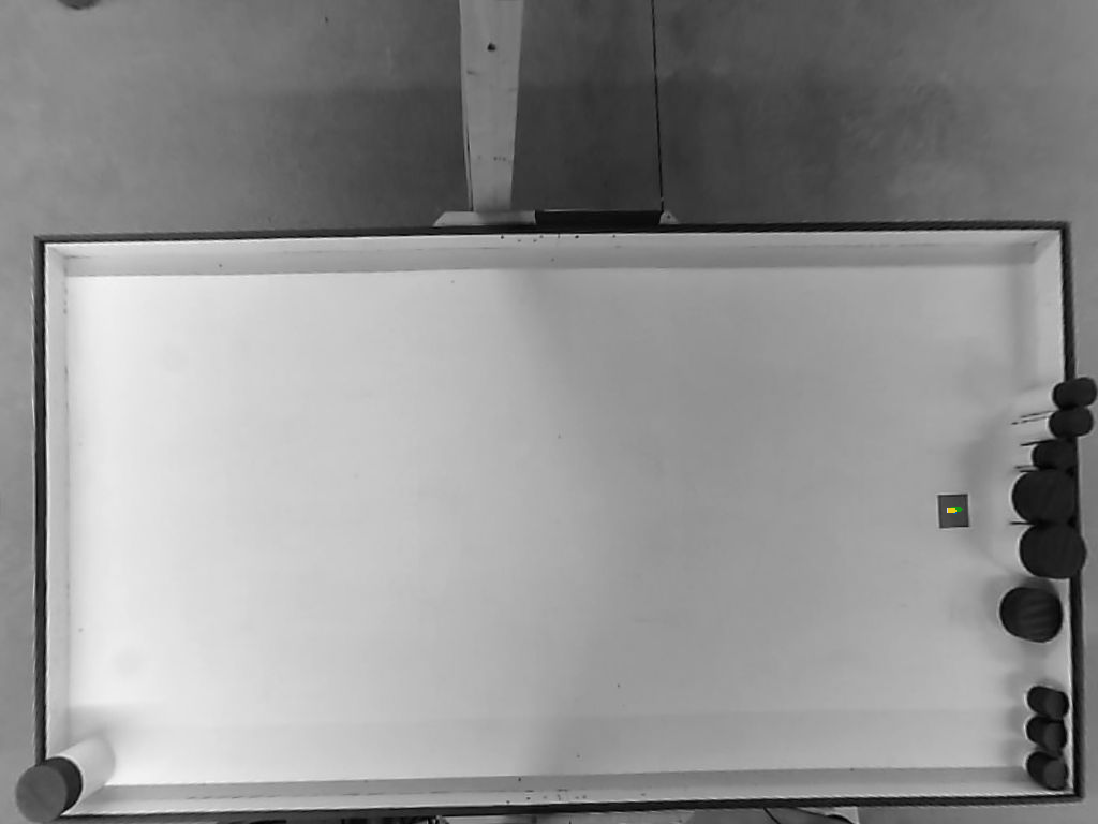
\includegraphics[width=\textwidth]{../hardwareX_paper/robot_8.png}
		\caption{Motion of blue tank \#8}
	\end{subfigure}
	\begin{subfigure}[t]{0.3\textwidth}
		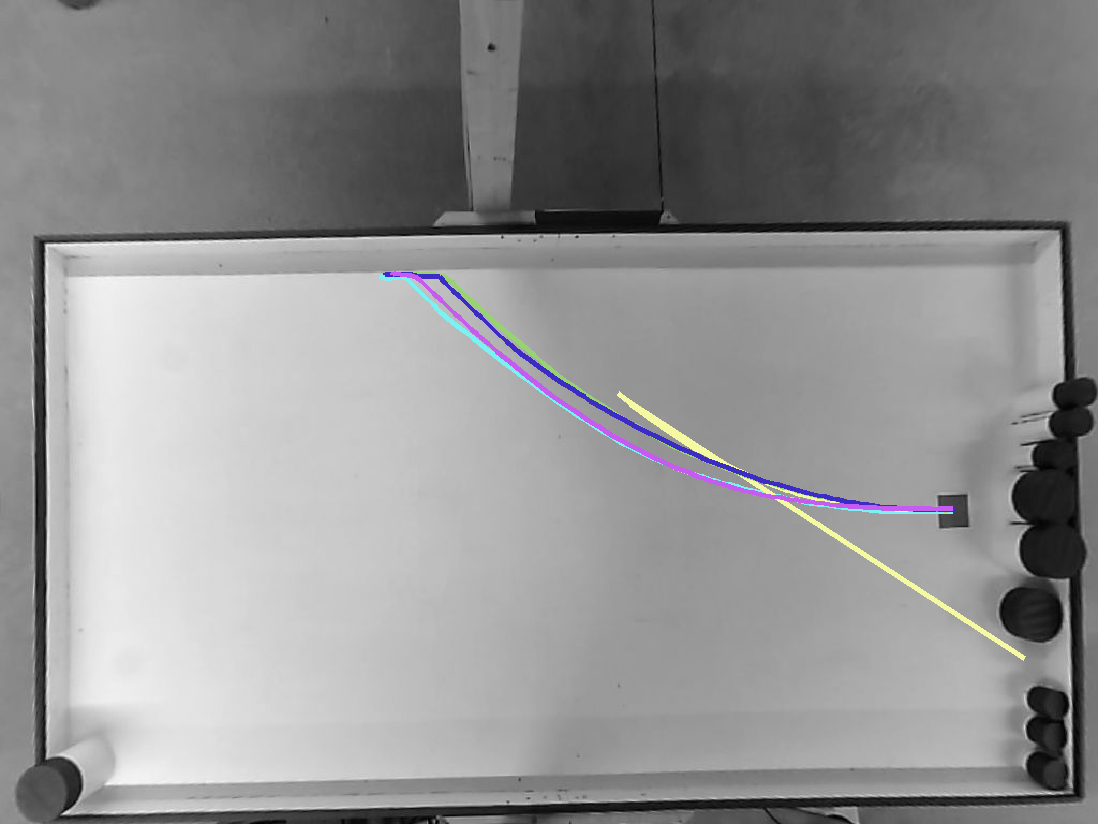
\includegraphics[width=\textwidth]{../hardwareX_paper/robot_18.png}
		\caption{Motion of blue tank \#18}
	\end{subfigure}
	
	\begin{subfigure}[t]{0.3\textwidth}
		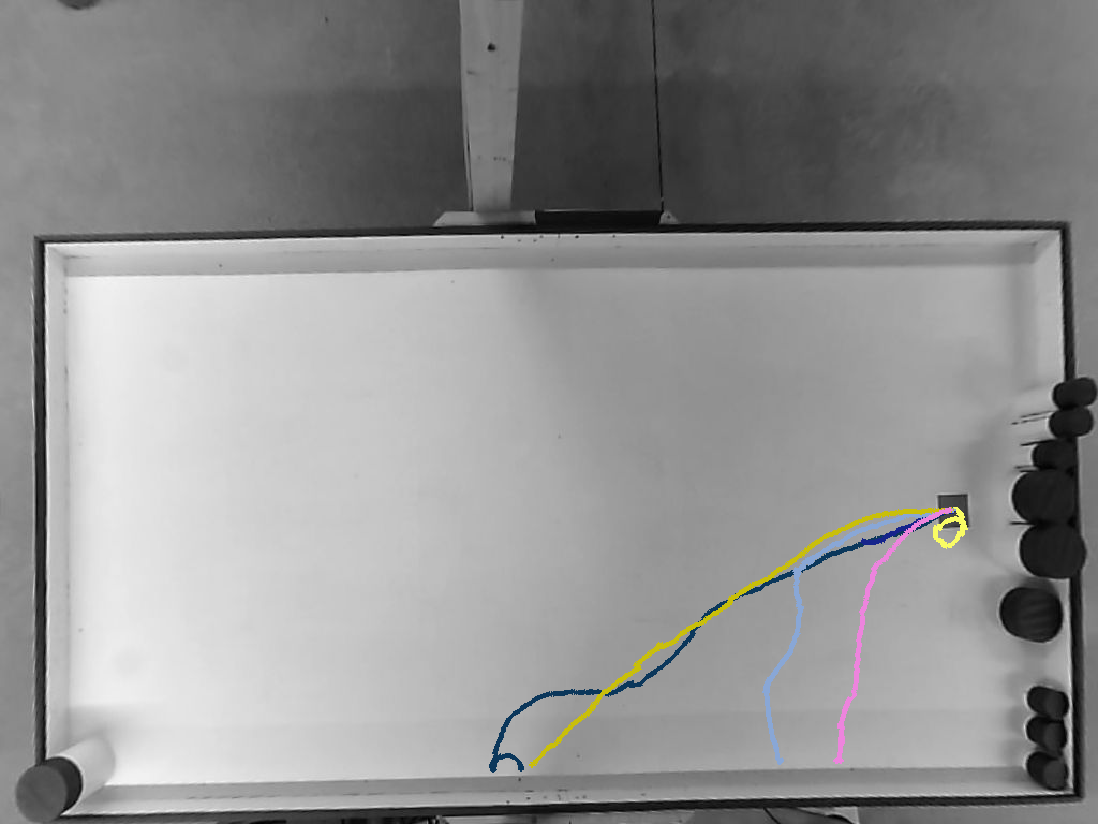
\includegraphics[width=\textwidth]{../hardwareX_paper/robot_5.png}
		\caption{Motion of bug robot}
	\end{subfigure}
	\label{img_traj}	
\end{figure}

The Hexbug-branded 6-wheeled bug (page \pageref{img_traj}, image c) displayed an asymmetry in its motor drive speeds. 
For three of its five runs, both motors ran, and the wheels on both sides rotated, but the right side was driven more quickly, and so the robot made a wide arc to the right and hit the wall of the arena behind the starting location. 
In one run, one side did not begin moving at all, causing the robot to rotate rapidly around that side. 
In another run, the robot twitched briefly, remained still, and then accelerated backwards quickly. 
This was likely caused by the gradual incrementing of the forward velocity eventually causing an integer overflow, resulting in a large forward velocity command being interpreted as a large negative velocity.

The green tank, carrying the number 0 AprilTag (page \pageref{img_traj}, image d), experienced problems with one side of its drive train in three of its five runs.
One tread drive did not move, while the other did, resulting in tight turns to the left in two runs, and to the right in one run. In one of the two remaining runs, the green tank did not move at all. In the second, the tank alternated movement and stopped periods until it reached the other side of the arena, which constituted success on this test. 

There are two blue tanks, carrying AprilTags numbered 8 and 18. 
Tank number 8 (page \pageref{img_traj}, image e) moved slightly on four of its 5 runs, and did not move on one of them. 
At no point did it move the full 0.25m. 
Tank number 18 (page \pageref{img_traj}, image f) moved much more consistently, but displayed an arc to the right in four of its 5 runs. 
In one run, the tank failed to restart after one of the stop phases, and eventually accelerated quickly in reverse. 
As with the 6-wheeled bug, this was likely the failure of the robot to move leading to a long enough delay that incrementing the commanded acceleration resulted in an integer overflow. 

The single-motor Hexbug-branded blue bug (page \pageref{img_traj}, image g) moved consistently, but with a heavy bias towards turning to the left. 
In every run, it started and stopped, but the curvature of the path to the left caused it to run into the left side of the arena. 
During one run, it fell over while moving, due to the somewhat ``bouncy'' nature of the toy's gait.

Some of these problems, such as the coasting of the Ackerman-steering car and the biases towards the left or right of some of the robots when commanded to move straight, can be overcome by software. 
For example, assuming the tags could be used to accurately measure the rotation of the robots, error between the detected rotational velocity and perceived rotational velocity could be accounted for in subsequent motion commands. 
The Ackerman-steering car drift could be reduced by sending a ``brake'' command to the motor driver IC to activate its back-EMF braking mode, rather than simply stopping by reducing the power output to zero. 
However, some of the problems are more difficult to alleviate. 
The tendency of the big wheel robot to flip over could be mitigated by very gradually increasing its speed, at the cost of reducing its control responsiveness, or by increasing the frequency of the feedback loop that checks its speed. 
Perhaps the blue bug would not fall over if its height were reduced, or the battery were placed lower on the body of the robot.
However, these mechanical problems could be more easily avoided by simply not using toys that have them. 

\subsection{Guidelines For Future Swarm Developers}
The origin of the TinyRobo hardware platform was a hobbyist project, intended to combine the diminishing cost and increasing power of Internet of Things (IoT) networking modules with the ready availability of toys to create a system that lowers the barrier to development of multi-robot systems.
While it did not fully achieve this goal, there are a number of lessons that will be relevant to future developers of multi-robot research platforms. 

The drivetrain of the system is of paramount importance. 
Sensors and networking can be virtualized, as in TinyRobo and GRITSBots, but no amount of clever programming will compensate for balky motion. 
The use of direct drive, as in GRITSBots or mROBerTO, is encouraged because the resulting drive train will be sealed against foreign matter. 
Further, the use of stepper motors in GRITSBots provides some degree of precision in motion control by directing the motor in steps of known resolution, rather than commanding a particular speed. 
If the system requires additional torque, sealed micro gearmotors can provide increased torque (although with reduction in speed), and will be more reliable than adopting a drivetrain from a toy. 

The chassis of the robot can be constructed from the same printed circuit board (PCB) that the electronics are supported on. 
Over the scales of forces present in tabletop swarms, PCB can be considered completely rigid, and electronics solder provides sufficient mechanical strength for motor mounts. 
The use of custom mechanical assemblies in e.g. Jasmine micro robots adds complexity to the build process. 
Where possible, small robots should be designed to use the PCB instead. 
Using children's toys in TinyRobo was intended to avoid the use of such custom parts, but brought with it additional problems that were outside of the scope of the work to solve, and could have been avoided with a simpler drivetrain. 

Parts count for small robots should be minimized.
TinyRobo was developed around the ESP-8266 WiFi module because the module includes both a powerful microprocessor and wireless communication. 
Multi-use devices like the ESP-8266 are becoming cheaper and more competent quickly.
The processor in mROBerTO is both a 32-bit ARM processor, a low-power Bluetooth transceiver, and an ANT Wireless tranceiver. 
The VL6180X IC combines an ambient light sensor and a laser-based time-of-flight range sensor in a package measuring approximately 5x8x1mm. 
Reducing parts count reduces cost and speeds assembly. 

Swarm robots should have autonomous charging, and have each robot be able to monitor its own battery level. 
Any operation that requires user intervention with each individual robot will not scale well as the swarm size increases. 
In the case of the Kilobots, the swarm as a whole can be charged in parallel, rather than requiring the individual robots to be connected with a charger. 
For the GRITSBbots, pins on the front of each robot allows the robot to connect to a charging station by itself, rather than requiring a human to connect it. 
The TinyRobo platform could be trivially altered to provide GRITSBots-style self-charging, but does not at present have a method to detect a low battery condition, aside from monitoring the motor drivers for an undervoltage signal. 
The alternative to this, leaving out self-charging and battery monitoring, results in increased effort by humans to keep the batteries charged and failures due to discharged batteries that are not immediately obvious to the control software. 
At a more general level, hardware health monitoring is required for systems that intend to detect their own failed components and work around them, which increases robustness in a swarm system. 

The latency and accuracy problems with AprilTags could be mitigated in a number of ways. 
First, the resolution of the camera can be increased while keeping the tags the same size and the camera the same distance away. 

This solution ends up requiring more computational power as the image size increases, in order to keep the tag detection framerate high enough to be useful for realtime control. 
AprilTags have very solid position and orientation tracking, but are computationally intensive to detect and localize in typical webcam images. 
More tags leads to longer computation time, increasing the latency of the robot control loop. 
Parallelizing the implementation of the AprilTag library could improve it significantly, but is out of scope for this work. 

One version of the GRITSBots used AprilTags and a standard web cam, resulting in position updates at approximately 10Hz. 
This update rate is consistent with that observed by the author using the ROS implementation of AprilTags. 
Decreasing the size of the image in which the tags are detected speeds it up, at the cost of requiring larger tags in order to have them legible in the lower-resolution image. 
The update rate places an upper bound on the ability of the system to respond to the motion of the robots. 
To decrease the latency of this sensing, the GRITSBots team considered moving to color blob tags, which can be detected by the onboard vision processor of a Pixy CMUCam5 at up to 50Hz \cite{PickemGrits2014}. 
MROBerTO also used color tracking, with a single RGB LED on top of each robot to identify it, and a green LED on the front of each robot to indicate its orientation. 
Kilobot robots also include an RGB LED, which may be set to any color by the software of the Kilobot. 
These LEDs can also provide swarm feedback in a manner similar to the LEDs in McLurkin's Swarmish interface \cite{mclurkin2006speaking}.

Second, the tag size could be increased, either by moving the tags closer to the camera and increasing their visual size, or by actually making the tags larger. 
Moving the camera closer reduces the useful area of the robot arena, and making the tags larger increases the size and weight of the robots, potentially overbalancing some of the less nimble robots. 
As was observed in the robot drive tests, the bug and big wheel bases were already prone to tipping over. 


%\section{Swarm Simulation} \label{section:Swarm_Simulation}
%
%Because the sensors in the TinyRobo system are simulated, it may appear that the development of the UI and translation components could have been served as well by a simulated swarm as by a real one. 
%This is not the case. 
%In 1992, Rodney Brooks pointed out that ``there is a vast difference (which is not appreciated by people who have not used real robots) between simulated robots and physical robots and their dynamics of interaction with the environment'' \citep{brooks1992artificial}. 
%The gap between real-world sensing and actuation and their simulated counterparts means that developers working solely in simulation are tempted to either invest effort in solving problems that do not occur in the real world, or fail to solve problems that do arise in the real world but are left out of simulation. 
%One of Brooks' examples, the directional nap of carpet having an effect on robot odometry that varied with direction of travel, is still not handled by modern physics simulators. 
%Even if it were handled, the attempt would over-complicate simulation configurations due to the variety of types of carpet available. 
%
%Modern simulators have vastly more powerful computers behind them than they did in 1992, and the development of video games with realistic physics models has contributed greatly to the variety of physics models available in modern robot simulators. 
%As of 2015, however, Brooks' point still holds, and the dynamics of robots interaction with the environment are still not perfectly simulated \citep{erez2015simulation}.
%Generally, aspects of physics are elided or approximated from gaming physics engines, in favor of rapid simulation which is visually plausible. 
%In particular, contact dynamics simulations are NP-hard, and so are approximated in the interests of speed. 
%The PhysiX and Havoc physics engines also do not implement Coriolis forces at all.
%These sorts of omissions are mostly harmless, but evolutionary techniques for developing controllers for robots or simulated creatures can exploit them to develop control schemes that cannot work under real physics \citep{Brooks2000}. 
%
%In the real world, sensors are also uncertain. 
%Simulated sensors can provide a level of accuracy and certainty about that accuracy that is not available to real sensors operating with the sensor noise that affects real-world systems. 
%As the TinyRobo system simulates its laser and distance sensors, it may appear that it falls into this trap of simulation, and provides sensors that are ``too good to be true''. 
%However, the TinyRobo sensors are physical sensors, they're just not the same physical sensors that they are presented as, in much the way that a sonar sensor is not a ruler, but rather measures time and sound and presents it as distance. 
%Similarly, the arena camera is not a robot-mounted laser scanner, but it is still a physical optical sensor being used to measure distance
%\todo{test noise of camera based fake laser vs real lasers, characterize difference between multiple sensor readings of same thing}
%Adding noise to simulated sensors can also move them more towards the sensors available on real robots, but as Brook's carpet nap example indicates, the type of noise may be more complex than a simple normal distribution about the ground truth value. 
%With evolutionary approaches, the system can even come to depend on the noise, and fail when it is given real sensors that are less noisy then their simulated counterparts \citep{jakobi1995noise} 
%%Tim Smithers, "On Why Better Robots Make it Harder"
%	The idea that the variation in real robot behavior will go away if the robots are "better" as a justification for simulation
%	Better-made components allowing hunting where worse ones provided damping (steam engine governor example)
%	Don't view robots as measuring with sensors and reasoning about results
%		Sensors act as filters whose output drives internal robot dynamics
%
%An Overview about Simulation and Emulation in Robotics
%Michael Reckhaus, Nico Hochgeschwender, Jan Paulus, Azamat Shakhimardanov and Gerhard K. Kraetzschmar
%	Simulation went out of fashion when people started getting real robots
%	Computers got better and games drive for realism pushed development
%	Proposes a lot of use cases and reasons to use simulation
%		Which are interestingly orthogonal to the reasons not to use it
%			One doesn't counter the other, it's just "here are the good parts, here are the bad parts"
%
%Simulation in robotics
%Leon Zlajpah
%	Overview of tools



